\section{EXP Exponential Function}

\subsection{Usage}

Computes the \verb|exp| function for its argument.  The general
syntax for its use is
\begin{verbatim}
   y = exp(x)
\end{verbatim}
where \verb|x| is an \verb|n|-dimensional array of numerical type.
Integer types are promoted to the \verb|double| type prior to
calculation of the \verb|exp| function.  Output \verb|y| is of the
same size and type as the input \verb|x|, (unless \verb|x| is an
integer, in which case \verb|y| is a \verb|double| type).
\subsection{Function Internals}

Mathematically, the \verb|exp| function is defined for all real
valued arguments \verb|x| as
\[
  \exp x \equiv e^{x},
\]
where
\[
  e = \sum_{0}^{\infty} \frac{1}{k!}
\]
and is approximately \verb|2.718281828459045| (returned by the function 
\verb|e|).  For complex values
\verb|z|, the famous Euler formula is used to calculate the 
exponential
\[
  e^{z} = e^{|z|} \left[ \cos \Re z + i \sin \Re z \right]
\]
\subsection{Example}

The following piece of code plots the real-valued \verb|exp|
function over the interval \verb|[-1,1]|:
\begin{verbatim}
--> x = linspace(-1,1);
--> plot(x,exp(x))
\end{verbatim}


\centerline{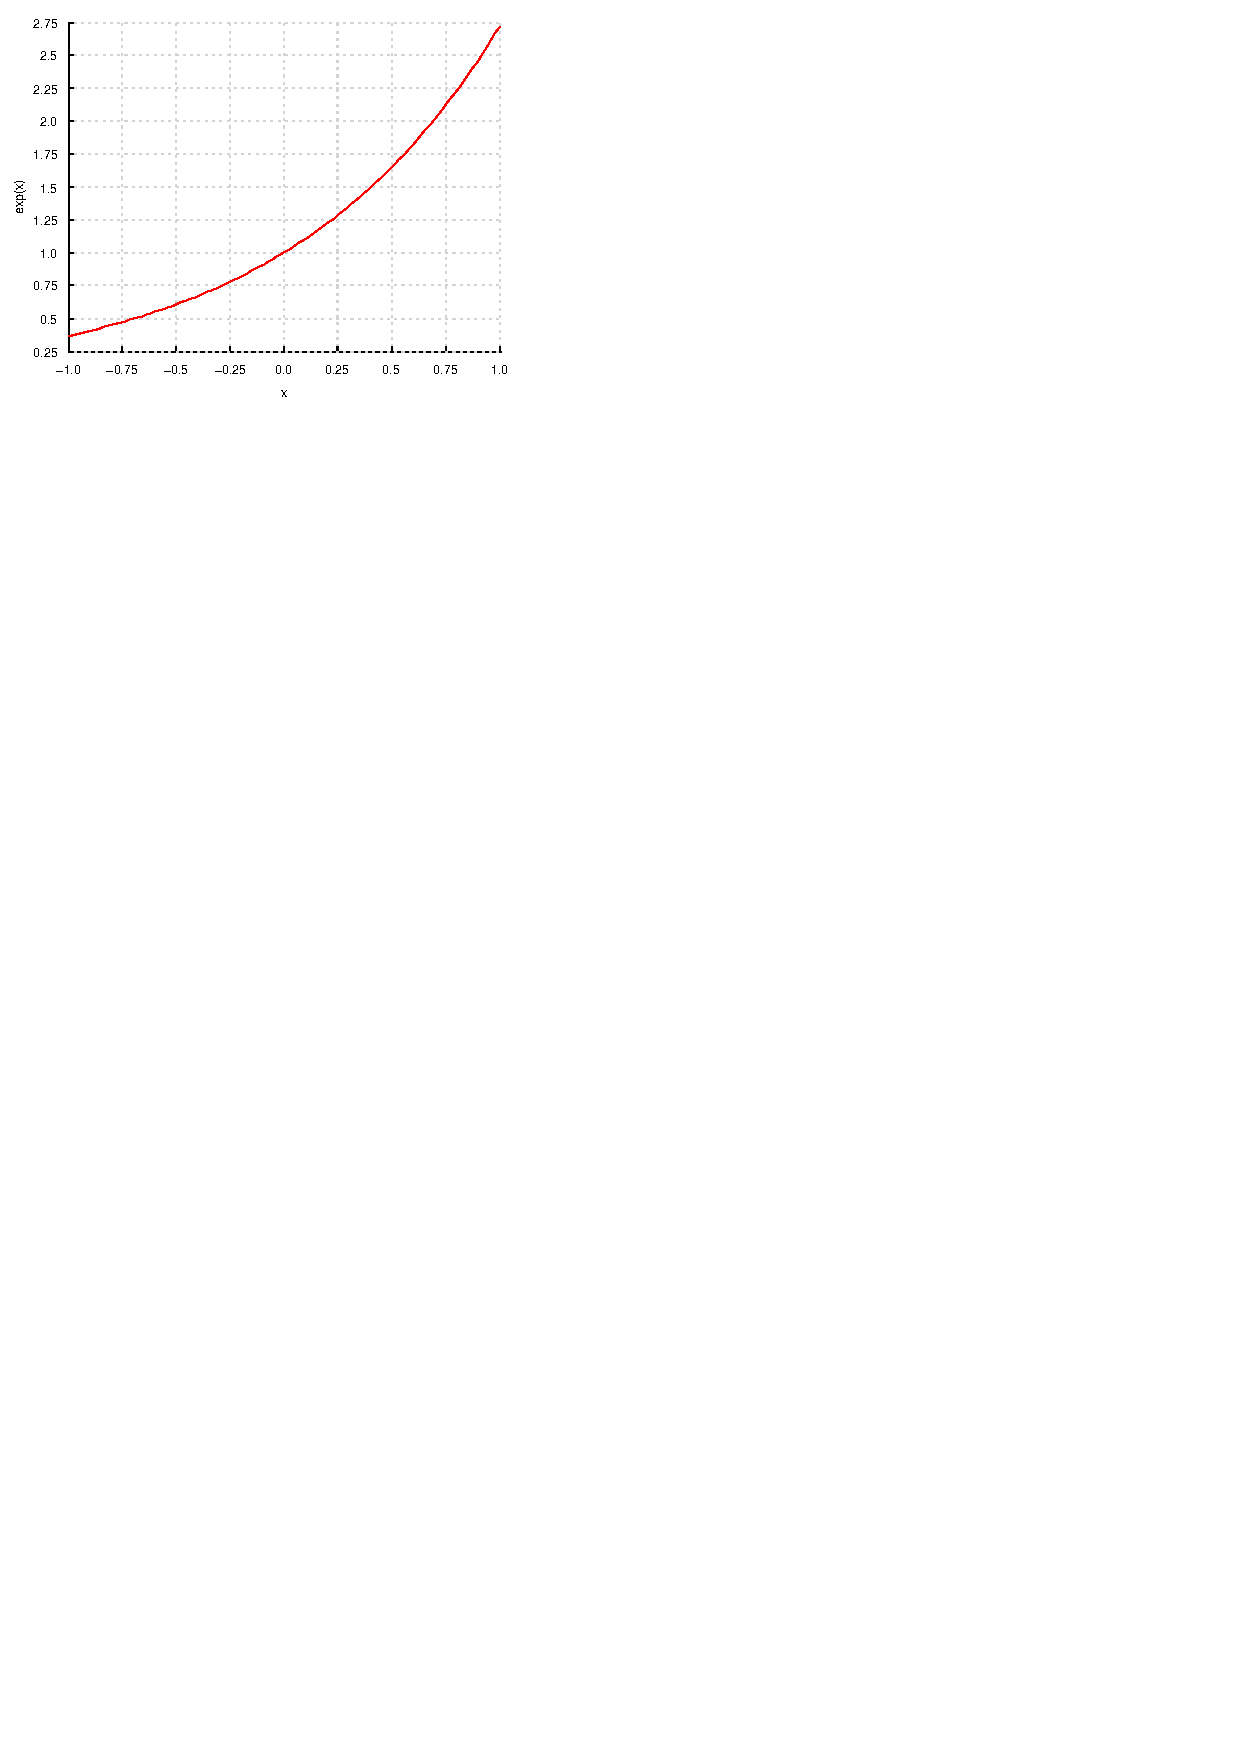
\includegraphics[width=8cm]{expplot1}}

In the second example, we plot the unit circle in the 
complex plane \verb|e\^{i 2 pi x}| for \verb|x in [-1,1]|.
\begin{verbatim}
--> x = linspace(-1,1);
--> plot(exp(-i*x*2*pi))
\end{verbatim}


\centerline{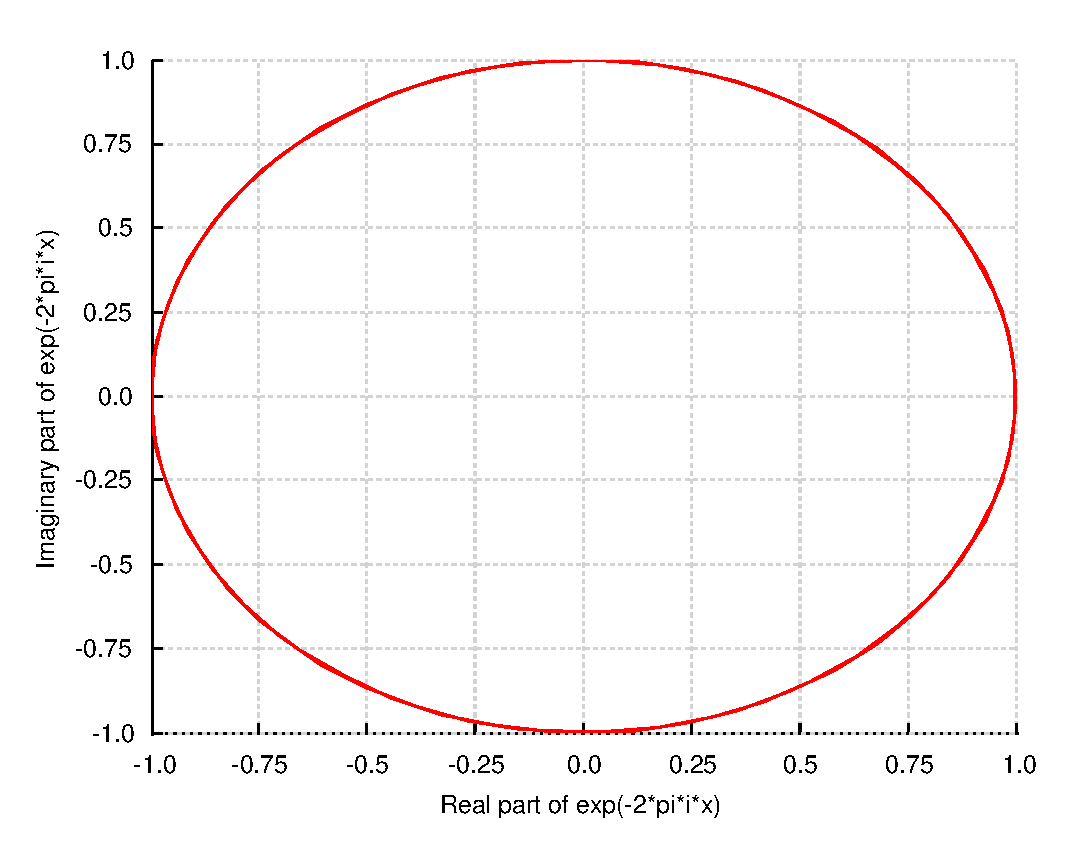
\includegraphics[width=8cm]{expplot2}}

